\chapterformat{Introduction}
Infrared (IR) spectroscopy is a widely used technique for the identification and characterization of chemical substances. Conventional Fourier Transform Infrared (FTIR) spectroscopy acquires absorption spectra by measuring the wavelength-dependent absorption of IR radiation by a sample. However, when analyzing extremely small sample masses below \SI{40}{\nano\gram}, as considered in this thesis, conventional approaches reach their sensitivity limits. Nanoelectromechanical systems (NEMS) for IR spectroscopy have demonstrated sensitivities in the nanogram and even picogram range \cite{Luhmann23}.

The subject of this thesis is a NEMS device for infrared spectroscopy consisting of a silicon nitride membrane (see Figure~\ref{fig:EMILIE}). During operation, the membrane and the deposited sample are irradiated with IR light and the sample absorbs significant amounts of light at characteristic wavelengths. This absorption causes a temperature increase in the sample, therefore heat is transferred to the membrane. By analyzing the resulting shift in the membrane’s eigenfrequencies as a function of wavelength, the absorption spectrum of the deposited molecules can be inferred \cite{Luhmann23}. This principle has already been successfully demonstrated, and the device is commercially available from Invisible-Light Labs under the name EMILIE \cite{Luhmann23,timaracpopovic25} (see section \ref{sec:emilie}). More precisely, the membrane is illuminated with a sweep of infrared wavelengths while its eigenfrequency response is continuously measured. To a good approximation, the silicon nitride membrane is transparent to IR light with the exception of one material specific absorption, such that absorption occurs almost exclusively in the sample material. When the sample absorbs IR light at a specific wavelangth, the local temperature of the membrane increases, leading to a softening of the stress and therefore reduction in its eigenfrequency. By analyzing the eigenfrequency response as a function of the IR excitation wavelength, an absorption spectrum of the sample material can be reconstructed.\\

Beyond absorption spectroscopy, the eigenfrequency response of the membrane also provides information about the spatial distribution of mass on its surface \cite{Hanay2012SingleproteinNM}. The membrane exhibits multiple eigenmodes with distinct mode shapes, as illustrated in Figure \ref{fig:modeshapes}. Depending on the geometrical position of the deposited material, different eigenmodes are affected to different degrees. By comparing the responses of several modes, the location of the additional mass on the membrane can be deduced. This concept is well established and has, for example, been demonstrated in \cite{Hanay2012SingleproteinNM}.\\

The aim of this thesis is to develop a numerical model of the membrane in order to predict the frequency response associated with given mass distributions. Such a model potentially enables the extraction of information about the mass and spatial distribution of material on the membrane from experimental measurements.\\

The simulations are carried out using the finite element method (FEM) with the open-source FEM package \ngsolve. 

\section{The EMILIE$^{\text{TM}}$ Device}
\label{sec:emilie}
The EMILIE$^{\text{TM}}$ device, developed by Invisible-Light Labs, is specifically designed for nanoelectromechanical fourier transform infrared spectroscopy (NEMS–FTIR). It consists of a prestressed $\silnit$ membrane integrated on a silicon chip and can be used in combination with a commercial Fourier Transform Infrared spectrometer (FTIR). The purpose of EMILIE$^{\text{TM}}$ is to detect and characterize chemical substances deposited on the membrane. As demonstrated in \cite{timaracpopovic25}, the device offers unique advantages, for example in the chemical characterization and monitoring of nanoplastics and ultrafine particles. An image of the chip and a commercial FTIR device used in combination with EMILIE$^{\text{TM}}$ is shown in Figure \ref{fig:EMILIE}.\\

\begin{figure}[h]
    \centering
    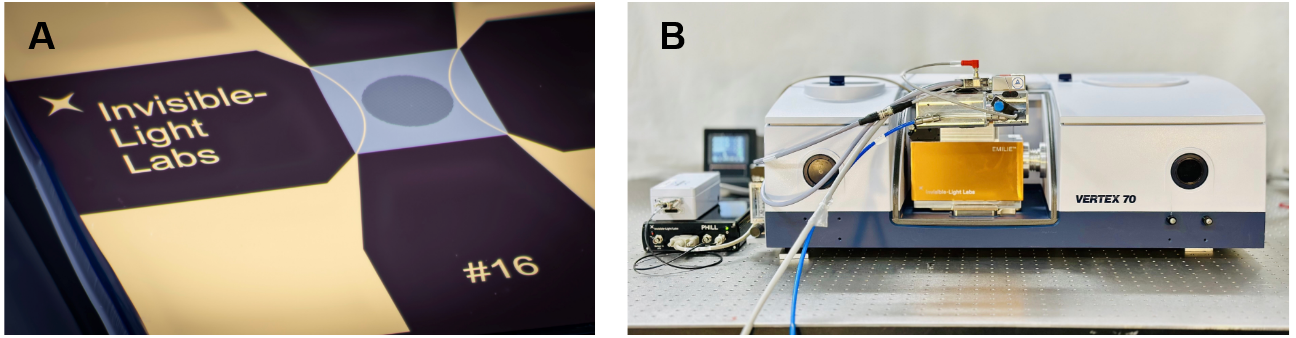
\includegraphics[width=\textwidth]{figures/pngs/EMILIE.png}
    \caption{\textbf{(A)} EMILIE device: a $\silnit$ membrane on a silicon wafer. \textbf{(B)} An FTIR spectrometer (Vertex 70, Bruker Corporation, MA, USA) equipped with the NEMS IR analyzer \cite{timaracpopovic25}.}
    \label{fig:EMILIE}
\end{figure}


% end of first translated section
\section{Notation}
In this chapter, the mathematical notation used throughout this thesis is defined.\\
Non-scalar variables such as vectors and matrices are written in boldface.\\
Differential operators are denoted by the nabla symbol $\nabla$. In particular, the gradient of a field is denoted by $\nabla$, and the divergence by $\nabla \cdot$.\\
The double contraction or double dot product ``$:$'' refers to the inner product of $N \times N$ matrices. For two matrices $\mathbf{A}$ and $\mathbf{B}$, it is defined as
\[
\mathbf{A}:\mathbf{B} = \sum_{i,j=0}^N A_{ij} B_{ij}.
\]\\
$\mathbf{1}$ and $\mathbf{0}$ denote the identity and zero elements, respectively, of the vector space under consideration.\\
The symbol $\partial$ preceding a set indicates the boundary of the set. More specifically, if a PDE is solved on a domain $\Omega$, then $\partial \Omega$ denotes the boundary of $\Omega$.\\
Densities are denoted by $\rho$, and stresses by $\sigma$. Since the problem is two-dimensional, densities have units of $kg/m^2$ and stresses have units of $N/m$. Whenever a physical density or stress with three-dimensional units ($kg/m^3$ or $N/m^2$) is used, this is indicated by the superscript ``3D.'' Similarly, the Young's modulus in 2D is denoted by $E$ with units of $N/m$. For a thin sheet of thickness $h$ and 3D Young's modulus $E^\mathrm{3D}$, the relation is $E = E^\mathrm{3D} \cdot h$.\\

\section{\ngsolve}
The FEM simulations in this thesis have been implemented using the software package NGSolve. Netgen/NGSolve is a high-performance multiphysics finite element software that is widely used in solid mechanics, fluid dynamics, and electromagnetics. Its flexible Python interface allows for the solution of the specific set of coupled PDEs considered in this thesis in a highly parameterized manner. Further information and documentation can be found in \cite{NGSolve}.\\

\section{Usage of LLMs}
Full disclosure: a large language model (LLM) has been used for the grammatical refinement of this thesis. At no point were the mathematical, physical, or empirical contents altered. The raw version of the thesis that was provided to the LLM will be made available under \url{https://zenodo.org/records/20592455} to allow verification that, aside from linguistic formulation, no scientific content was changed. The LLM used was ChatGPT5 by OpenAI. The prompt employed was:\\
\\
I will provide you with a section of my master's thesis in LaTeX format. Please revise the text to improve its clarity, grammar, and scientific tone, transforming it into proper scientific English suitable for an academic thesis in computational science and technology.

Important instructions:

- Do not alter any mathematical, physical, or empirical content, equations, variable names, or references.

- If you find any mathematical mistakes please make me aware of them but do not conduct any changes.

- Maintain all LaTeX commands and formatting.

- Focus on improving sentence structure, clarity, word choice, and formal tone.

- Avoid redundant expressions and make the language more concise where appropriate.

- Keep the formatting and structure unchanged unless needed for clarity.

- Anything labeled "TODO" will be changed afterwards. Leave it as it is.

- If there are any larger changes that you would suggest like restructuring, let me know but do not change right away.

Once you're ready, I’ll begin by pasting the raw LaTeX content.

\section{Code}
The code used in this thesis is available at \url{https://github.com/tobias-slowiak/msc}. The simulation itself, along with numerous utility functions, is implemented in the main file \texttt{emilie\_simulation.py}. The code is designed to be executed in Jupyter notebooks, with all data-generating code contained in the files \texttt{notebooks/*.ipynb}. Each notebook is also converted into a standard Python script using \texttt{scripts/convert\_notebooks.py}, resulting in the scripts \texttt{scripts/*.py}. Certain features, such as \ngsolve visualizations generated with the function \texttt{draw\_on\_mesh}, are not available in the converted scripts.\\
To reproduce the plots in this thesis, run \texttt{scripts/run\_all.py}. The plots corresponding to section \ref{sec:parameter_search} are excluded from this script, as they require more computational resources. These can instead be generated by running \texttt{scripts/parameter\_search.py}. The physically relevant part of the code is also included in section \ref{sec:appendixB}.\\

\newpage
